\documentclass[border=6pt]{standalone}
\usepackage{tikz}
\usetikzlibrary{arrows.meta,positioning,calc,shapes.geometric,fit,backgrounds,patterns,matrix,decorations.pathreplacing}
\begin{document}
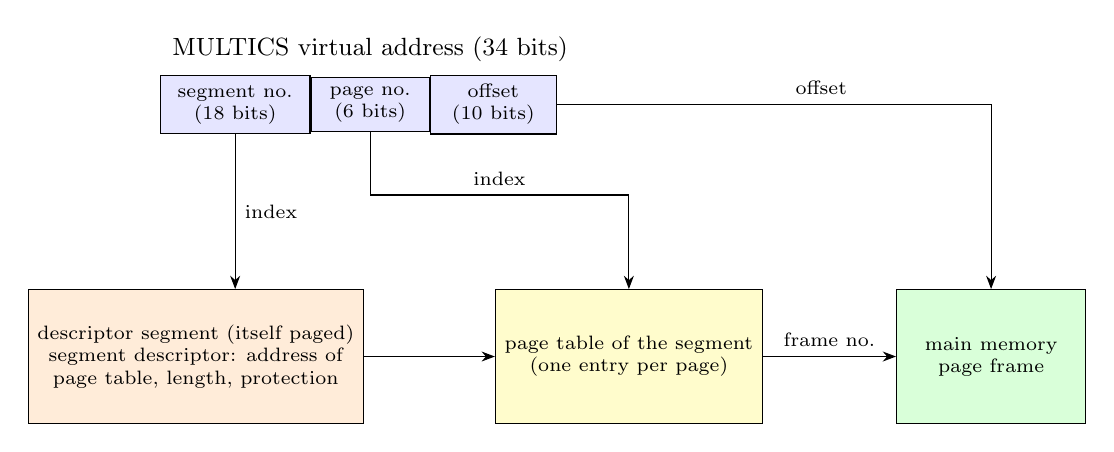
\begin{tikzpicture}[>=Stealth,font=\small]
\tikzstyle{b}=[draw,minimum height=0.6cm,font=\scriptsize,align=center]
\node[b,minimum width=1.9cm,fill=blue!10] (s) at (0,0) {segment no.\\ (18 bits)};
\node[b,minimum width=1.5cm,fill=blue!10,right=0pt of s] (p) {page no.\\ (6 bits)};
\node[b,minimum width=1.6cm,fill=blue!10,right=0pt of p] (o) {offset\\ (10 bits)};
\node[above=2pt of p,font=\small] {MULTICS virtual address (34 bits)};
\node[b,minimum width=3.6cm,minimum height=1.7cm,fill=orange!15] (ds) at (-0.5,-3.2) {descriptor segment (itself paged)\\ segment descriptor: address of\\ page table, length, protection};
\node[b,minimum width=3.2cm,minimum height=1.7cm,fill=yellow!20] (pt) at (5.0,-3.2) {page table of the segment\\ (one entry per page)};
\node[b,minimum width=2.4cm,minimum height=1.7cm,fill=green!15] (mem) at (9.6,-3.2) {main memory\\ page frame};
\draw[->] (s.south) -- (s.south |- ds.north) node[midway,right,font=\scriptsize]{index};
\draw[->] (ds.east) -- (pt.west);
\draw[->] (p.south) -- ++(0,-0.8) -| (pt.north) node[pos=0.25,above,font=\scriptsize]{index};
\draw[->] (pt.east) -- node[above,font=\scriptsize]{frame no.} (mem.west);
\draw[->] (o.east) -- ++(1.2,0) -| (mem.north) node[pos=0.25,above,font=\scriptsize]{offset};
\end{tikzpicture}
\end{document}
